%% TeXworks instructions:
% !TeX root = ./report.tex
% !TEX encoding = UTF-8 Unicode
%% !TEX program = arara
%% !TEX TS-program = arara
% !TeX spellcheck = it-IT

% arara: pdflatex: { synctex: yes, action: batchmode, options: "-halt-on-error -file-line-error-style" }
% arara: pdflatex: { synctex: yes, action: nonstopmode, options: "-halt-on-error -file-line-error-style" }

%% Generate a report.xmpdata file with title and authors for PDF/A-compliant format %%
\begin{filecontents*}{\jobname.xmpdata}
    \Title{Maraph1-mp Project Report}
    \Author{Nicholas Brasini\sep Gjulio Jakova\sep Federico Naldini\sep Jacopo Riciputi}
\end{filecontents*}

\documentclass[%
    a4paper,            % specifica il formato A4 (default: letter)
    10pt,               % specifica la dimensione del carattere a 10
    oneside,            % serve per impaginare per stampa solo fronte
    notitlepage         % mette il titolo in una pagina separata (solo per article)
]{article}

\usepackage{a4wide}             % consente di avere più spazio nell'A4

%% ORDINE IMPORTANTE INIZIO %%%%%%%%%%%%
\usepackage[T1]{fontenc}        % serve per impostare la codifica di output del font
\usepackage{textcomp}           % serve per fornire supporto ai Text Companion fonts
\usepackage[utf8]{inputenc}     % serve per impostare la codifica di input del font
\usepackage[
    english,            % utilizza l'inglese come lingua secondaria
    italian             % utilizza l'italiano come lingua primaria
]{babel}                        % serve per scrivere Indice, Capitolo, etc in Italiano

\usepackage{lmodern}            % carica una variante Latin Modern prodotto dal GUST
%% ORDINE IMPORTANTE FINE %%%%%%%%%%%%%%

\usepackage{indentfirst}        % serve per avere l'indentazione nel primo paragrafo
\usepackage{setspace}           % serve a fornire comandi di interlinea standard
\usepackage{xcolor}             % serve per la gestione dei colori nel testo
\usepackage{graphicx}           % serve per includere immagini e grafici
\setcounter{figure}{0}
\renewcommand{\thefigure}{\arabic{section}.\arabic{figure}} % serve a cambiare la didascalia dell'immagine basandosi sulla sezione in cui è chiamata

\graphicspath{{./images/}}

\usepackage[%
    strict,             % rende tutti gli warning degli errori
    autostyle,          % imposta lo stile in base al linguaggio specificato in babel
    english=american,   % imposta lo stile per l'inglese
    italian=guillemets  % imposta lo stile per l'italiano
]{csquotes}                     % serve a impostare lo stile delle virgolette

\usepackage{multirow}           % aggiunge la possibilità di raggruppare celle su più righe nelle tabelle

\onehalfspacing%                % Imposta interlinea a 1,5 ed equivale a \linespread{1,5}

\setcounter{secnumdepth}{4}     % Numera fino alla sottosezione nel corpo del testo
\setcounter{tocdepth}{4}        % Numera fino alla sotto-sottosezione nell'indice

\usepackage[%
    depth=3,            % equivale a bookmarksdepth di hyperref
    open=false,         % equivale a bookmarksopen di hyperref
    numbered=true       % equivale a bookmarksnumbered di hyperref
]{bookmark}                     % Gestisce i segnalibri meglio di hyperref
\usepackage{hyperref}           % Gestisce tutte le cose ipertestuali del pdf
\hypersetup{%
    pdfpagemode={UseNone},
    hidelinks,          % nasconde i collegamenti (non vengono quadrettati)
    hypertexnames=false,
    linktoc=all,        % inserisce i link nell'indice
    unicode=true,       % only Latin characters in Acrobat’s bookmarks
    pdftoolbar=false,   % show Acrobat’s toolbar?
    pdfmenubar=false,   % show Acrobat’s menu?
    plainpages=false,
    breaklinks,
    pdfstartview={Fit},
    pdfauthor={Nicholas Brasini, Gjulio Jakova, Federico Naldini, Jacopo Riciputi},
    pdfcreator={Nicholas Brasini, Gjulio Jakova, Federico Naldini, Jacopo Riciputi},
    pdftitle={Maraph1-mp Project Report},
    pdflang={it}
}
\usepackage[utf8]{inputenc} % serve per avere l'indice di tutti i capitoli all'inizio

%\usepackage[a-1b]{pdfx}
\usepackage[%
    english,italian,    % definizione delle lingue da usare
    nameinlink          % inserisce i link nei riferimenti
]{cleveref}                     % permette di usare riferimenti migliori dei \ref e dei varioref

\title{\LARGE{\textbf{Maraph1-mp Project Report}}}

\author{%
    Nicholas~Brasini\\%
    Gjulio~Jakova\\%
    Federico~Naldini\\%
    Jacopo~Riciputi
}

\date{%
    \small{Paradigmi di Programmazione e Sviluppo}\\%
    \small{Anni accademici 2017--2018 e 2018--2019}
}


\begin{document}

    \maketitle
    \clearpage
	\tableofcontents
	\clearpage
    \section*{\Huge {Capitolo 1}\label{chapter1}}
      \section{Processo di sviluppo}\label{sec:process}
        \subsection {Metodologia di sviluppo}\label{subsec:metodology}
        \subsection {Strumenti adottati}\label{subsec:tools}

        \clearpage

    \section*{\Huge {\textbf Capitolo 2}\label{chapter2}}
    \section{Requisiti}\label{sec:requirements}
         \subsection {Requisiti utente}\label{subsec:requirements:business}
             \subsection {Requisiti funzionali}\label{subsec:requirements:functional}
            \subsubsection[Gioco]{\large {Regole del gioco}\label{subsub:requirements:game}}
            \subsubsection[NoAutenticazion]{\large {Servizio di gioco senza autenticazione}\label{subsub:requirements:noauth}}
            \subsubsection[Autenticazion]{\large {Servizio di gioco con autenticazione}\label{subsub:requirements:auth}}
            \subsubsection[Stanze di gioco]{\large {Servizio delle stanze di gioco}\label{subsub:requirements:lobby}}
            \subsubsection[Interfaccia utente]{\large {Interfaccia grafica per l'utente}\label{subsub:requirements:gui}}
        \subsection {Requisiti non funzionali}\label{subsec:requirements:notFunctional}
        \subsection {Requisiti implementativi}\label{subsec:requirements:implementative}

   \clearpage

    \section{Design architetturale}\label{sec:design}
        \subsection[Architettura]{Architettura e pattern utilizzati}\label{subsec:architecture}
            \subsubsection{Architettura server-side}\label{subsub:architecture:server}
            \subsubsection{Architettura client-side}\label{subsub:architecture:client}
        \subsection{Tecnologie}\label{subsec:technologies}

        \clearpage

    \section{Design di dettaglio}\label{sec:details}

	In questa senzione saranno presentate le scelte effettuate a livello di desing nel dettagio. In primo luogo si tratterà dell'organizzazione generale del codice in \texttt{packages} e dei \textit{design patters} applicati più frequentemente, successivamente saranno analizzati nel particolare le principali classi di ogni modulo del sistema, presentando eventuali pattern di desing caratteristici di quella classe.

    \subsection {Organizzazione del codice}\label{subsec:details:codestructure}
    La struttura del progetto si presenta divisa in cinque \texttt{packages} principali, tre di questi corrispondono perfettamente agli elementi principali dell'architettura distribuita del sistema, i restanti due sono stati pensati come supporto ai principali.

    \begin{itemize}
    \item{\texttt{client:\/}} All'interno del \texttt{package} client viene modellata l'interazione tra un utente fruitore del gioco e
    l'architettura remota del sistema, sono presenti quindi tutte le classi necessarie alla realizzazione dell'interfaccia grafica, al supporto delle funzionalità lato client di gioco, ricerca e aggiunta di un amico, replay e visualizzazione in tempo reale di una partita.


    \item{\textbf{\texttt{discovery:\/}}}
      Questo \texttt{package} contiene tutti i sorgenti relativi all'implementazione del \textit{discovery server},
      server centralizzato che espone un servizio di pagine gialle: consente cioè di mantenere traccia di tutti i \textit{server} attivi
      all'interno del sistema, nonchè di tutte le partite che stanno venendo disputate e dei giocatori online.

    \item{\texttt{server:\/}}
      Il \texttt{package} server comprenede i file necessari a mettere in gioco un server backend per gestire le partite,
      il login e la registrazione degli utenti, il salvataggio in remoto dei punteggi e delle partite.

    \item{\texttt{commons:\/}}
      Uno dei due \texttt{packages} di supporto: contiene un insieme di classi e oggetti di \textit{utilities} comuni agli altri \texttt{packages} del sistema.

    \item{\texttt{core:\/}}
      Il secondo \texttt{package} che non corrisponde direttamente a un elemento dell'architettura distribuita, contiene il cuore del sistema, ovvero l'implementazione delle regole e logiche di gioco Marafone; nonostante potesse essere inserito all'interno di uno degli altri \texttt{packages}, si è scelto di mantenerlo separato, in quanto contenente un'insieme di classi ed oggetti ad alto valore per il sistema.

  \end{itemize}

  \subsection {Pattern di progettazione generali}\label{subsec:details:generaldesingpattern}
  Durante l'intero processo di sviluppo e integrazione sono stati impiegati diversi \textit{desing patterns}, tra questi alcuni si sono prestati meglio di altri a un applicazione costante e ripetuta all'interno di varie strutture.\\
  Il primo e più utilizzato tra tutti i \textit{patterns} è stato sicuramente il \texttt{Factory Method}: avendo infatti deciso di utilizzare
  il linguaggio di Programmazione \textit{Scala} come principale linguaggio impiegato all'interno del progetto, è venuto abbastanza naturale adattare il processo di definizione dei metodi di una classe UML alla generazione di un \texttt{trait} e di realizzare la sua implementazione a una classe privata all'interno del \texttt{Companion Object} del trait in questione, mettendo a disposizione il metodo \texttt{apply()} di tale oggetto come \texttt{Factory Method}
  Un altro pattern decisamente impiegato è stato il pattern \texttt{Strategy}, grazie all'approccio orientato al paradigma funzionale del linguaggio \textit{Scala}, è venuto molto naturale definire classi e strutture che isolassero alcuni algoritmi necessari per il loro funzionamento e permettessero di definirli dinamicamente.
  Infine è utile citare, sebbene non ricada strettamente in all'interno di una specifica categoria di \textit{desing patterns}, la scelta di desing effettuata nel realizzare insiemi di oggetti statici: invece di utilizzare una struttura basata sulle enumerazioni, si è deciso di sfruttare i costrutti messi a disposizione dal linguaggio scala, ottenendo una soluzione composta da un \texttt{trait} che definisse il contratto da rispettare e una serie di \texttt{case objects} estendenti il \texttt{trait}.

  \subsection {Core}\label{subsec:details:core}
  Punto di partenza per il desing del sistema è stata la descrizione delle funzionalità e componenti necessarie allo svolgimento di una partita di Marafone, come mostrato dal relativo diagramma delle classi nella figura 4.1.

\begin{figure}[htbp]
  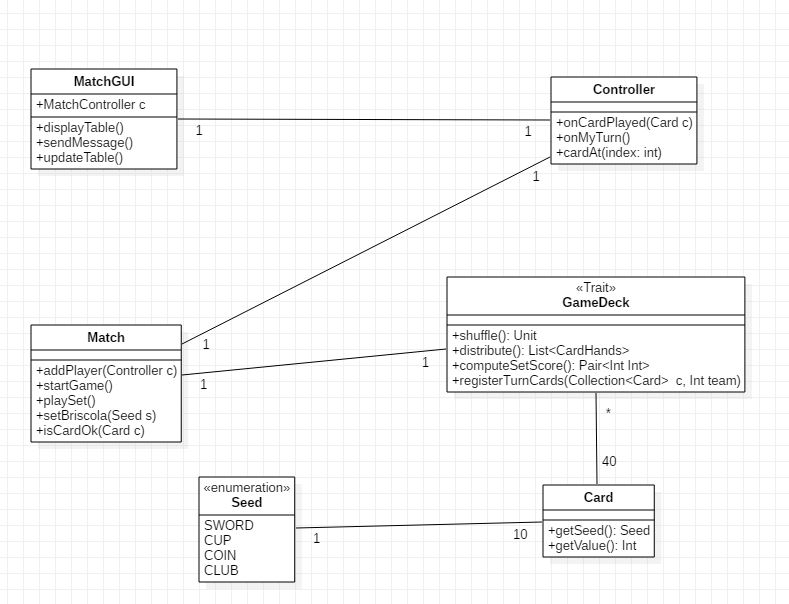
\includegraphics[width=\textwidth,height=\textheight,keepaspectratio]{initialArchitecture}
   \caption{diagramma delle classi relativo allo svolgimento di una partita}
\end{figure}

 E' importante sottolinare che tale diagramma rappresenta una visione di alto livello del sistema dal punto di vista esclusivamente della modellazione di una partita, non catturando in nessun modo caratteristiche legate ad altri domini quali la separazione del sistema secondo un modello distribuito, tuttavia posto che alcuni elementi sarebbero stati realizzati mettendo in gioco scelte di desing piuttosto complesse, il modello fornito dallo schema risultava piuttosto solido.
 Come è possibile notare, lo schema si struttura seguendo il pattern di progettazione \textit{MVC}, dove i componenti soggetti a una maggiore complessità risultano sicuramente controller e view, mentre model risulta più solido e definito.
 Di conseguenza si è scelto di catturare all'interno del \texttt{package core} la componente di modello della partita, identificandone i principali componenti:

\begin{itemize}
  \item{\texttt{mazzo di gioco:\/}} all'interno del package \texttt{deck} sono presenti tutte le strutture e funzionalità necessarie alla gestione del mazzo di gioco, come ad esempio la divisione delle carte nelle mani dei giocatori e il mescolamento delle stesse all'interno del mazzo; viene definita inoltre la struttura necessaria per la registrazione e calcolo del punteggio durante la partita.


  \item{\texttt{ciclo di gioco:\/}} il package \texttt{game} contiene l'insieme delle regole e procedure che regolano una partita tra quattro giocatori, definendo inoltre i concetti di set, team e match.

  \item{\texttt{giocatore:\/}} definisce il concetto di giocatore e le operazioni possibili da parte di quest'ultimo.

\end{itemize}

  Per quanto riguarda le funzionalità di controller e gui, esse sono state realizzate all'interno di core in un primo momento, ma sono poi state integrate nei moduli più adeguati al loro utilizzo.

\subsection {Discovery}\label{subsec:details:discovery}
All'interno del \texttt{package discovery} si è realizzato il servizio di discovery, seguendo i requisiti e le specifiche definite in fase di progettazione dell'architettura distribuita.\\
In quanto elemento unico e comune a tutta l'architettura, il discovery server svolge le funzioni di un registro centralizzato, consultabile e aggiornabile da ogni altro componente del sistema, tale registro deve mantenere quindi i riferimenti ai server online, il numero di partite al momento disputate all'interno del sistema, un loro identificativo e il server su cui sono eseguite, inoltre tiene traccia dei giocatori online che hanno effettuato il login, fornendo la possibilità agli altri giocatori di contattarli.
Mostrato nella figura 4.2, è possibile vedere il diagramma delle classi relativo al \texttt{package discovery}

 \begin{figure}[htbp]
  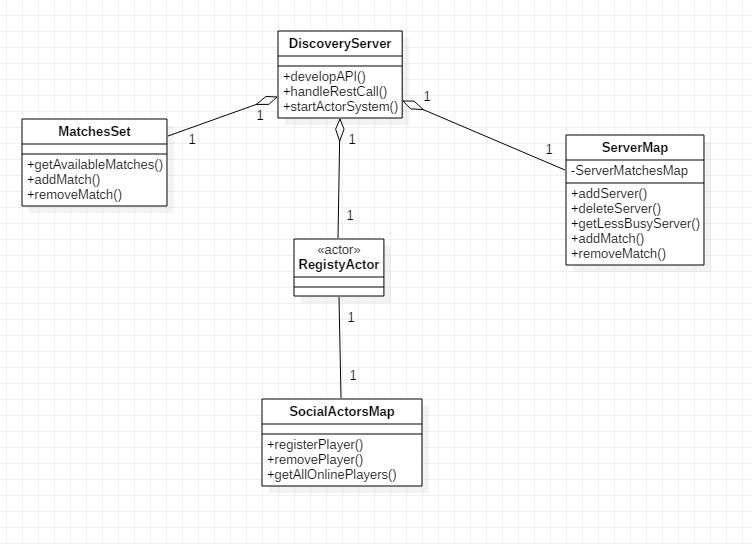
\includegraphics[width=\textwidth,height=\textheight,keepaspectratio]{discoveryArchitecture}
   \caption{diagramma delle classi relativo alla struttura del discovery}
  \end{figure}

Tale diagramma presenta una classe al centro \texttt{DiscoveryServer} e tre classi in relazione di composizione con essa.
La prima tra queste è \texttt{MatchesSet}, classe che mette a disposizione una semplice struttura per gestire all'interno del discovery l'insieme delle partite giocate in tempo reale, salvandone l'identificatore.\\
Successivamente \texttt{RegistryActor} realizza un attore che gestisce un oggetto di classe \texttt{SocialActorsMap}, questo attore comunica con tutti i \texttt{SocialActor} presenti all'interno del sistema mediante il protocollo \textit{Publish-Subscribe} messo a disposizione dalla libreria \textit{Akka cluster}, ricevendo richieste di registrazione e rimozione di utenti e pubblicando una versione aggiornata della lista degli utenti online sul canale.//
In secondo luogo è presente \texttt{SocialActorsMap}: tale classe incarna una struttura praticamente analoga a \texttt{MatchesSet}, con l'unica differenza di gestire il riferimento ai giocatori online invece che alle partite.\\
Infine \texttt{ServerMap} gestisce l'elenco dei server disponibili, tenendo conto anche del numero di partite disputato sopra di esse.\\
Elemento chiave per l'intero package è sicuramente \texttt{DiscoveryServer}, classe che realizza l'implementazione di un server web ,estendendo le classi \texttt{Verticle} della libreria \textit{Vertx}, e delle \textit{Rest API} necessarie per contattarlo.
Menzione particolare meritano le \textit{Rest API}, sviluppate come \texttt{case objects} estendenti un \texttt{trait} chiamato \texttt{RestAPI}, presente nel \texttt{package commons}. Il contratto definito da tale \texttt{trait} vincola ogni oggetto a implementare tre metodi:
\begin{itemize}
  \item{\texttt{path:\/}} definisce il path necessario per richiamare la \textit{Rest API} all'interno del server su cui viene esposta.

  \item{\texttt{httpMethod:\/}} specifica il methdo http con cui deve essere effettuata la chiamata.

  \item{\texttt{asRequest:\/}} crea un oggetto della classe \texttt{Request} a partire dalla \textit{Rest API}, tale classe consente di specificare tramite uno \texttt{strategy method} le operazioni da eseguire quando viene ricevuta una richiesta corrispondente all'API in questione.
\end{itemize}

Questa progettazione delle API consente un aggiunta dinamica e facile di nuove API a quelle già presenti, per aggiungere una nuova api non occorre fare altro che definire un oggetto estendente il trait \texttt{DiscoveryAPI} e un handler per la richiesta generata da tale API all'interno del metodo \texttt{deployAPI}
Le API attualmente presenti su discovery sono le seguenti.

\begin{itemize}
  \item{\texttt{RegisterServer:\/}} registra un server all'interno del discovery.

  \item{\texttt{GetServer:\/}} API chiamata da client, restituisce il server su cui al momento, sono attive meno partite, implementando così una basilare forma di \textit{load balance} all'interno del sistema.

  \item{\texttt{RegisterMatch:\/}} API chiamata da un server, registra l'id di una nuova partita sul discovery e aggiorna il contatore delle partite in corso relative al singolo server.

  \item{\texttt{RemoveMatch:\/}} API chiamata da un server, notifica al discovery la fine di una partita, rimuovendo il suo id dal discovery e aggiornando il contatore relativo al server.

  \item{\texttt{RegisterSocialID:\/}} API chiamta da un client dopo la fase di autenticazione, notifica a \texttt{RegistryActor} la presenza di un nuovo subscriber da contattare.
\end{itemize}

Oltre all'esposizione delle seguenti API, il discovery ha anche il compito di mettere in esecuzione i \textit{seed nodes} necessari per \textit{Akka cluster}, si è scelto infatti di posizionare i \textit{seed nodes}, ovvero due \texttt{ActorSystem} che fungono da \textit{entry points} all'interno del sistema cluster, sopra lo stesso host in cui viene messo in esecuzione il server, così da accentuare ulteriormente il carattere centralizzato del discovery server.\\
 A tal proposito è necessario citare il metodo \texttt{startDiscoveryCluster}, che dato l'indirizzo ip della macchina su cui viene messo in esecuzione il discovery server, costruisce due \texttt{ActorSystem} sulle porte 2551 e 2552 che creano la struttura di cluster al cui interno si andranno a inserire gli \textit{ActorSystem} in esecuzione sui vari client e server.

 \subsection {Server}\label{subsec:details:server}
 Questo è il modulo contenente tutto il codice necessario a mettere in esecuzione un server backend. Le funzionalità esposte da questo server sono di creazione e gestione di varie partite, competitive o meno, di registrazione e autenticazione di utenti, di salvataggio e recupero di partite terminate.Oltre a queste operazioni che rispondono direttamente a una richiesta di un utente, sono presenti anche tutta una serie di procedure di comunicazione con il discovery server, in modo da mantenere sempre lo stato di quest'ultimo aggiornato con lo stato effetivo del sistema.
 Ogni server è pensato per essere indipendente da gli altri server, delegando le politiche di selezione e divisione del lavoro al discovery Server:
 E' infatti importante notare che ogni client non contatta uno specifico server al momento dell'avvio, ma contatta il discovery server, il quale provvederà a assegnargli uno tra i server con minor numero di partite al momento disputate; questa scelta ci è parsa ragionevole in quanto il numero di partite al momento effettuate poteva fornire un primo, per quanto instabile, indice di carico computazionale del singolo server, di conseguenza andare a selezionare di volta in volta un server diverso per ogni client che si univa al sistema poteva essere un semplice, seppur rozzo, meccanismo di \textit{load balance} all'intero del sistema.\\
 La figura 4.3 riassume efficacemente i passaggi che portano all'esecuzione di una chiamata REST all'interno di un server da parte di un client.\\

 \begin{figure}[htbp]
   \includegraphics[width=\textwidth,height=\textheight,keepaspectratio]{restApiCall}
    \caption{diagramma di sequenza relativo all'esecuzione di una chiamata rest}
 \end{figure}

 Queste modalità comunicative sono utilizzate per tutte le interazioni tra client e server, fatta eccezione per le comunicazioni durante la partita, in tale frangente si è scelto di affidarsi alla comunicazione real time tra attori tramite messaggi end to end e il protocollo \textit{publish subscribe} messo a disposizione da \textit{Akka cluster}.
 Principale e più importante funzionalità del server è la creazione, gestione, distuzione delle varie istanze delle partite in gioco:
 alla chiamata di una specifica \textit{Rest API} chiamata \texttt{FoundGameAPI} viene avviato il processo di ricerca di una nuova partita; per prima cosa vengono estrapolati dall'interno della richiesta il nome utente del giocatore che ha inviato la richiesta e eventuali nomi di avversari/compagni, tali dati vengono poi spediti a un attore, \texttt{LobbyActor} con il compito di mantenere la lista delle lobby, ovvero delle partite di gioco con numero di giocatori insufficenti a iniziare una nuova partita, nel caso tra le lobby ve ne sia una che può ospitare tutti i giocatori della richiesta, allora essi sono aggiunti a tale lobby, altrimenti viene creata una nuova lobby, determinata la lobby, all'utente viene infine notificato l'identificatore della lobby in cui è stato inserito. \\
 Nel momento in cui una lobby raggiunge il numero massimo di giocatori viene dato il via a una nuova partita:in primo luogo il server notifica al discovery l'incremento del numero di partite in esecuzione, successivamente viene creato un attore di classe \texttt{GameActor} a cui vengono passati gli identificatori dei quattro giocatori che prenderanno parte alla partita; tale attore ha il compito di gestire lato server la partita, andando a fornire a ogni giocatore le sue carte, applicando le regole per la gestione della briscola, delle mani, del punteggio e così via.\\
 Come affermato sopra, le comunicazioni durante la partita avvengono tramite scambio di messaggi tra il \texttt{GameActor} e gli attori dei quattro giocatori, in particolare \texttt{GameActor} pubblica messaggi su un canale a cui gli altri quattro attori sono iscritti, mentre riceve messaggi spediti dal singolo attore.
 Al momento della fine di una partita, il server si occupa di registrarla su un database remoto, di aggiornare il discovery e rimuovere la lobby dalla propria lista interna.\\
 Descritte le modalità di gestione delle partite, tutti gli altri servizi presenti sul database sono di ricerca e/o aggiunta di nuovi dati a un database backend, tramite un meccanismo a \textit{Rest API}, di seguito è riportato l'elenco delle principali \textit{Rest API} sviluppate all'interno del server:
 \begin{itemize}
   \item{\texttt{FoundGame:\/}} comincia la ricerca di una partita secondo le modalità sopra descritte, la richiesta di questa API può contenere al suo interno da uno a quattro username e un flag che specifica se si andrà a giocare una partita competitiva o meno.

   \item{\texttt{AddUser:\/}} registra un nuovo utente sul database backend con le credenziali specificate nella richiesta.

   \item{\texttt{LoginUser:\/}} controlla se le credenziali fornite da un utente durante il login corrispondono a quelle salvate all'interno del database.

   \item{\texttt{GetUser:\/}} recupera dal database i dati relativi a un utente,tra cui il punteggio attuale dell'utente.

   \item{\texttt{AddFriend:\/}} aggiunge alla lista degli amici dell'utente che effettua la richiesta un nuovo amico.

    \item{\texttt{GameRest:\/}} recupera dal database una partita registrata.

    \item{\texttt{GetFriends:\/}} recupera dal database la lista degli amici dell'utente che effettua la richiesta.
 \end{itemize}

 Ognuna di queste API fa riferimento a un oggetto della classe \texttt{RedisUserUtils} che si occupa di generare, gestire e recuperare il risultato delle queries necessarie allo svolgimento delle operazioni richieste.

  \subsection {Client}\label{subsec:details:client}
  Tra tutti i \texttt{packages} del progetto, sicuramente \texttt{Client} risulta quello più complesso e articolato.Nonostante discovery e server catturino una buona parte della complessità dei requisiti del sistema, una parte altrettanto grande, se non maggiore è delegata a questo modulo.\\
  \texttt{Client} si pone il difficile compito di offrire all'utente fruitore del gioco tutte le funzionalità da lui attese gratificandolo con una valida \textit{User experience}, mascherando il più possibile la complessità dovuta all'itegrazione e supporto con le altre componenti del sistema.

  \begin{figure}
    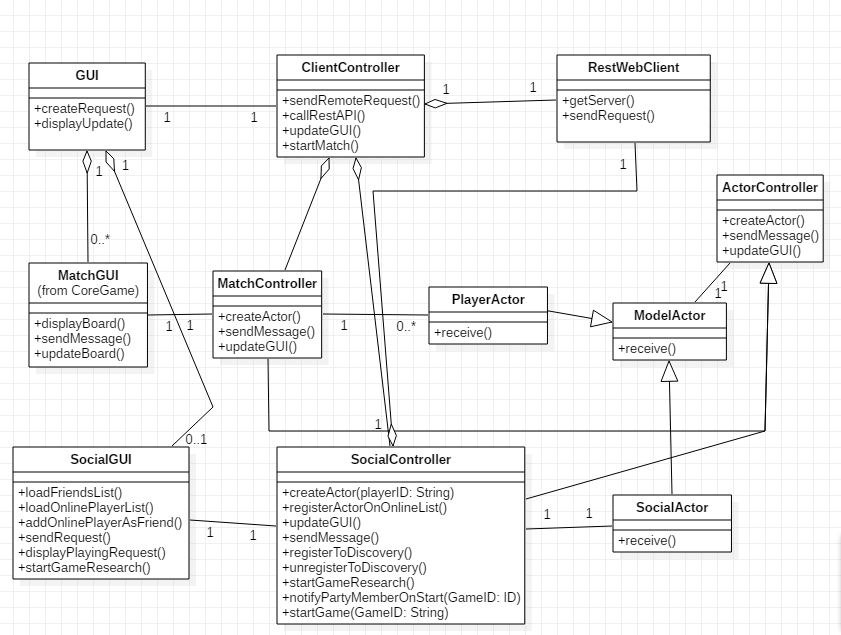
\includegraphics[width=\textwidth,height=\textheight,keepaspectratio]{clientArchitecture}
     \caption{diagramma delle classi relativo al package client}
  \end{figure}

  La struttura del \texttt{package} segue quella del classico modello di progettazione \textit{MVC}, occorre però precisare che dentro model sono contenute principalemente le classi necessarie alla comunicazione remota con server e discovery, la parte di modello effettivo del sistema gestito all'interno del client è minimale, come previsto dall'architettura client server.











    \clearpage

    \section{Implementazione}\label{sec:implementation}
        \subsection{Nicholas Brasini}\label{subsec:brasini}
        \subsection{Gjulio Jakova}\label{subsec:jakova}
        \subsection{Federico Naldini}\label{subsec:naldini}
        \subsection{Jacopo Riciputi}\label{subsec:riciputi}

        \clearpage

    \section{Retrospettiva}\label{sec:retrospective}

\end{document}
